\documentclass[10pt, conference]{IEEEtran}
\usepackage[T1]{fontenc}
\usepackage[utf8]{inputenc}
\usepackage[english]{babel}
\usepackage[usenames]{color}
\usepackage{colortbl}
\usepackage{graphicx}
\usepackage{array}
\usepackage{multirow}
\usepackage{booktabs}
\usepackage{subfig}
\usepackage{float}
\usepackage[obeyspaces,hyphens,spaces]{url}
\usepackage{balance}
\usepackage{amsmath}
\usepackage{tikz}
\usetikzlibrary{positioning,arrows.meta}
\pagenumbering{arabic}
\pagestyle{empty}
\clubpenalty = 10000
\widowpenalty = 10000
\displaywidowpenalty = 10000
\usepackage{cleveref}

\makeatletter
\renewcommand{\paragraph}[1]{\noindent\textsf{#1}.}
\makeatother

\newcommand{\tpl}[1]{\texttt{\small #1}}

\title{Log Representations and Learning Regimes for Log-based Anomaly Detection: A Replication and Extension Study}
\author{Pham Minh Dung Duong (2553085)$^{1}$, Thanh Nghiep Quan (2557078)$^{1}$, Tran Vo (2553737)$^{1}$
    \\
    \emph{$^{1}$ Dep. of Computer and Software Engineering, Polytechnique Montréal, Canada}}

\begin{document}
\maketitle

\begin{abstract}
\textit{Context:} Machine learning models for log-based anomaly detection need the raw logs to be parsed and turned into numbers. Wu et al.~\cite{wu2023effectiveness} studied how this log representation step affects the models.
\textit{Objective:} We replicate their first research question for two supervised models on two datasets. We also check whether removing correlated features helps. We then extend the study on one dataset with an unsupervised and a semi-supervised model, a statistical ranking, and an explanation of the best model.
\textit{Method:} We parse HDFS and BGL with Drain and the preprocessing of Qin et al. We train a Random Forest on message count vectors and an LSTM on BERT template embeddings, with and without correlation and redundancy analysis. On HDFS we add PCA (unsupervised) and LogGPT (a GPT-2 model trained on normal sessions only). We retrain the four models on 10 random train/test splits, rank them with the Scott-Knott ESD test, and explain the best model with SHAP.
\textit{Results:} The Random Forest results are reproduced (F1 0.999 on HDFS, 0.919 against 0.891 on BGL). The LSTM is better than reported on HDFS (0.987 against 0.959), which we trace to a windowing bug in the original code, and worse on BGL (0.870 against 0.931). Removing correlated features does not improve accuracy. On HDFS, the ranking is RF $>$ LSTM $>$ LogGPT $>$ PCA for both F1 and AUC. LogGPT reaches a mean F1 of 0.856 from 5,000 normal sessions, and its F1 depends on its Top-K threshold. SHAP shows that the Random Forest relies mostly on one error template and on the number of events of the block write pipeline.
\textit{Conclusion:} On HDFS, a supervised model on simple count features gives the best results. Without labels, the threshold and the training protocol matter as much as the model.
\end{abstract}

\section{Introduction}
\label{sec:introduction}

Software systems write logs that record what happens at run time. When a failure occurs, engineers often look at these logs first. Because modern systems produce millions of log lines, automated log-based anomaly detection has been studied widely~\cite{he2016experience,du2017deeplog}. Most approaches follow the same pipeline: the raw log lines are parsed into event templates, grouped into sequences (sessions), represented as numeric features, and given to a model that labels each session as normal or anomalous.

Wu et al.~\cite{wu2023effectiveness} studied the representation step of this pipeline. In their RQ1 they compared six representations with seven models on four datasets. They found that the choice of representation has a non-negligible effect on the results, that the simple Message Count Vector (MCV) performs best overall, and that BERT embeddings work best for models that use the order of events. This report presents a partial replication and an extension of that work. It answers four research questions:

\begin{itemize}
\item \textbf{RQ1 (replication):} Can we reproduce the RQ1 results of Wu et al. for a classical and a deep learning supervised model on HDFS and BGL?
\item \textbf{RQ2 (feature selection):} Does removing correlated and redundant features change the performance of the classical model?
\item \textbf{RQ3 (extension):} How do an unsupervised and a semi-supervised model compare with the two supervised models when all four are trained and tested under the same protocol?
\item \textbf{RQ4 (explanation):} Which log events drive the decisions of the best model, and are these explanations stable?
\end{itemize}

Our replication found three issues in the original replication package that change the reported numbers. We fixed them and measured the effect of each one. All the code, configuration files, and result files that produce the numbers in this report are in our replication package (folders \texttt{part1/} and \texttt{part2/}). Every design decision is logged there with its reason (\texttt{DECISIONS.md}).

\section{Approach}
\label{sec:approach}

\Cref{fig:pipeline} gives an overview. Part 1 (RQ1, RQ2) uses HDFS and BGL. Part 2 (RQ3, RQ4) uses HDFS only.

\begin{figure*}[t]
\centering
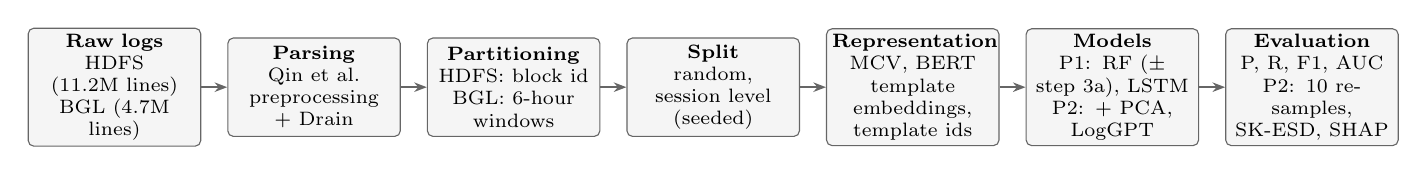
\begin{tikzpicture}[
  box/.style={draw=black!60, rounded corners=2pt, fill=black!4, align=center, font=\scriptsize,
              text width=2.05cm, minimum height=1.25cm, inner sep=2pt},
  arr/.style={-{Stealth[length=1.6mm]}, black!60, thick}, node distance=0.33cm]
\node[box] (raw) {\textbf{Raw logs}\\HDFS (11.2M lines)\\BGL (4.7M lines)};
\node[box, right=of raw] (parse) {\textbf{Parsing}\\Qin et al. preprocessing + Drain};
\node[box, right=of parse] (part) {\textbf{Partitioning}\\HDFS: block id\\BGL: 6-hour windows};
\node[box, right=of part] (split) {\textbf{Split}\\random, session level\\(seeded)};
\node[box, right=of split] (rep) {\textbf{Representation}\\MCV, BERT template embeddings, template ids};
\node[box, right=of rep] (model) {\textbf{Models}\\P1: RF ($\pm$ step 3a), LSTM\\P2: + PCA, LogGPT};
\node[box, right=of model] (eval) {\textbf{Evaluation}\\P, R, F1, AUC\\P2: 10 resamples, SK-ESD, SHAP};
\foreach \a/\b in {raw/parse, parse/part, part/split, split/rep, rep/model, model/eval} \draw[arr] (\a) -- (\b);
\end{tikzpicture}
\caption{Overview of our pipeline. P1 = Part 1 (replication, HDFS and BGL); P2 = Part 2 (extension, HDFS).}
\label{fig:pipeline}
\end{figure*}

\subsection{Datasets}

We use two of the four datasets of the original study, both from Loghub~\cite{zhu2023loghub} (\cref{tab:data}). \textbf{HDFS}~\cite{xu2009detecting} comes from a Hadoop file system. Each log line refers to a data block, and each block is labelled normal or anomalous by the dataset authors. \textbf{BGL}~\cite{oliner2007supercomputers} comes from a BlueGene/L supercomputer, where each line has its own label (alert or not). We chose these two because they are widely used in the literature and they differ in a useful way. HDFS has many short sessions with few anomalies, while BGL has long windows and many anomalies. The line counts match the original study (11,175,629 and 4,747,963 lines).

\begin{table}[t]
\centering
\caption{Datasets after parsing and partitioning}
\label{tab:data}
\footnotesize
\setlength{\tabcolsep}{2.2pt}
\begin{tabular}{lrrrrrr}
\toprule
 & Templates & Sessions & Anomalous & Events/sess. & Train & Test \\
\midrule
HDFS & 47 & 575,061 & 16,838 (2.9\%) & 19.4 & 402,542 & 172,519 \\
BGL & 421 & 826 & 409 (49.5\%) & 5,748.1 & 660 & 166 \\
\bottomrule
\end{tabular}
\end{table}

\subsection{Log parsing}

We parse the logs with Drain~\cite{he2017drain} (depth 4, similarity threshold 0.5, at most 100 children), the parser used by the original study. Before parsing, we apply the preprocessing framework of Qin et al.~\cite{qin2025preprocessing}, as suggested by the assignment. It masks variable parts (IP addresses, paths, block ids, numbers) with 14 ordered regular expressions. It first checks which expressions match the first 2,000 lines and then applies only those to the whole file. We reused the authors' code without changes. Block ids (HDFS) and labels and timestamps (BGL) are extracted before masking. We obtain 47 templates for HDFS (the original study reports 46) and 421 for BGL.

To check the parsing quality, we ran the same pipeline on the Loghub-2.0 samples of 2,000 lines with corrected ground truth~\cite{jiang2024loghub2}. Grouping accuracy was 1.000 on HDFS and 0.970 on BGL. This is equal to or higher than Drain with the regular expressions used by the original study (0.998 and 0.970). Grouping accuracy matters most for count features, because two lines in the same group are counted as the same event.

\subsection{Partitioning and splitting}

For HDFS, one session contains all lines that mention the same block id, in log order. For BGL, we use fixed, non-overlapping 6-hour windows, as in the original study. A window is anomalous if at least one of its lines is labelled as an alert. This gives 826 windows, while the original paper reports 718. We tried several variants (aligning windows to the epoch, using another time field, removing small windows), but none gives 718. The original code does not include the windowing step, so we kept the literal definition of the paper. As in the paper, we split the sessions at random (70/30 for HDFS, 80/20 for BGL) with a fixed seed. Our HDFS split sizes are exactly the ones of the paper. The main runs use seed 42. To measure the variance, we also repeat Part 1 with seeds 0 to 4.

\subsection{Representations}

\paragraph{Message Count Vector (MCV)} One feature per template counts how many times it appears in the session. The vocabulary is built from the training sessions only, and events of templates never seen in training are dropped. We use MCV for the Random Forest because the original study found it to be the best representation for classical models. We also use it for PCA, which was designed for count matrices~\cite{xu2009detecting}.

\paragraph{BERT embeddings} Each template text is given to the pre-trained \texttt{bert-base-uncased} model~\cite{devlin2019bert}. Its embedding is the mean of the token vectors of the second-to-last layer (768 dimensions, at most 50 tokens). These settings follow the original replication package. A session becomes a sequence of these vectors, which the LSTM reads in order. In the original study, BERT gave the best results for the models that use the order of events in 7 of 8 cases, and it gives the LSTM some knowledge of the meaning of each event.

\paragraph{Why these pairings} We pair the level of each representation with the mechanism of the model, as Wu et al.~do: ``all of our studied traditional models take sequence-level representation as input'', while ``LSTM models require fixed length event-level representation as input''~\cite{wu2023effectiveness} (\S4.3.1). For the RF we use MCV because it is exactly the fixed-dimension, order-free feature vector that a forest of CART trees consumes~\cite{breiman2001random}, and because the original study ranks it first: in their SK-EST test, the three classical representations ``outperformed their semantic-based counterparts, with MCV achieving the best rank''~\cite{wu2023effectiveness} (\S5.1). For the LSTM we use BERT embeddings because each of its ordered input positions needs a dense, context-aware vector: ``the BERT embedding is ranked first in the deep-model-only ranking'' and ``achieves the best performance for 7 out of the 8 cases of the models that can leverage sequential information''~\cite{wu2023effectiveness} (\S5.1). PCA keeps the event count matrix it was designed for---Xu et al.~``adopt the unsupervised dimension reduction method PCA with event count matrix to detect anomalies''~\cite{wu2023effectiveness,xu2009detecting} (\S3.1). LogGPT, finally, reads the raw template-id sequence: its GPT-2 backbone learns its own representation internally, being trained to predict the next template id of normal sessions~\cite{han2023loggpt}.

\subsection{Supervised models (Part 1)}

\paragraph{Random Forest (RF)} A classical model~\cite{breiman2001random}, robust to irrelevant features and fast to train. We use the settings of the replication package: 10 trees, $\sqrt{p}$ features per split, no depth limit, no class weights. The anomaly score is the predicted probability of the anomalous class.

\paragraph{LSTM} A deep learning model~\cite{hochreiter1997lstm} that can use the order of events. We use the architecture of the package: one LSTM layer with 8 hidden units, a linear output layer, cross-entropy loss, Adam with learning rate $10^{-3}$, 30 epochs, and balanced sampling of the sessions. Sessions are cut into sliding windows (size 30, step 1 for HDFS; size 50, step 50 for BGL). Every window gets the label of its session, and the session score is the highest anomaly probability of its windows.

\paragraph{Changes to the replication package} We found three issues in the package and fixed them:
(1) For RF, the metric function is called with its arguments swapped, so the printed precision is the recall and vice versa.
(2) For sessions shorter than the window, the package keeps only the last $w-L-1$ events of a session of length $L$. With $w=30$, a session of 19 events (the HDFS median) keeps 10 events. We feed whole sessions and use packed sequences, so padding never reaches the last hidden state.
(3) The package keeps the epoch with the best F1 on the test set. We hold out 10\% of the training sessions and select the epoch on this validation set.
We also train in mini-batches of 512 windows instead of one optimizer step per session, because the latter would take several hours per run on HDFS. To measure the effect of these changes, we ran ablations that reproduce the package's windowing and training (\cref{sec:rq1}).

\subsection{Correlation and redundancy analysis (step 3a)}

Correlated features can split the importance of one underlying event across several features and make a model harder to interpret. We apply the analysis to the RF features, using the training data only. First, we compute the Spearman correlation between all features and cluster them hierarchically (average linkage, distance $1-|\rho|$). We cut the tree at 0.3 ($|\rho| \geq 0.7$) and keep, in each cluster, the template that occurs most often. Second, we repeatedly remove the feature with the highest variance inflation factor (VIF) until all VIFs are at most 5. We do not apply this step to the LSTM. Its 768 inputs are embedding dimensions, not events, and the embedding matrix of the 47 HDFS templates has rank 47. Most dimensions are therefore exact linear combinations of others, so every VIF would be infinite.

\subsection{Unsupervised and semi-supervised models (Part 2)}

Labelled anomalies are rare and costly in practice, so we add two models that do not need them. They come from two different categories, as required.

\paragraph{PCA (classical, unsupervised)} PCA~\cite{xu2009detecting} is the classical baseline for count features. We port the implementation of loglizer~\cite{he2016experience} and keep its defaults. The MCV is weighted with TF-IDF and centred, both fitted on the training data. We keep the principal components that explain 95\% of the variance. The anomaly score of a session is its squared prediction error (SPE), i.e., the squared length of its projection on the remaining (residual) components. A session is anomalous if the SPE is above the Q-statistic threshold at $\alpha=0.001$~\cite{jackson1979control}. PCA is trained on the whole training split with the labels removed, so about 2.9\% of its training sessions are anomalous.

\paragraph{LogGPT (LLM-based, semi-supervised)} LogGPT~\cite{han2023loggpt} trains a small GPT-2 model~\cite{radford2019gpt2} from scratch (6 layers, 6 heads, embedding size 60) to predict the next template id of normal sessions. During testing, a session is anomalous if, at any position, the actual next template is not among the $K$ most likely predictions. A template never seen in training counts as a miss. We chose LogGPT because it represents the LLM-based category, its code is public, and it is small enough to train on a laptop GPU. As in the paper, it is trained on 5,000 normal sessions sampled from the training split (labels are used only for this filter): 4,500 for training and 500 for validation. Pre-training runs for 100 epochs (learning rate $10^{-4}$, batch size 16). It is followed by reinforcement learning (RL) fine-tuning with a Top-K reward: $+1$ when the actual next template is in the Top-K, $-1$ otherwise (learning rate $10^{-6}$, at most 20 episodes, early stopping on the validation loss). $K$ is 50\% of the unique templates of the training sessions, rounded down.

We ported the authors' code to current PyTorch and fed it the same template sequences that the LSTM sees, instead of using its own parser. Where the code and the paper disagree, we followed the code. The paper describes the RL step as PPO~\cite{schulman2017ppo}, but the code makes one policy-gradient update per generated sequence, without the PPO ratio and clipping. The code also uses the last pre-training epoch, not the one with the best validation loss (on our runs the difference in validation loss is at most 1.2\%). We removed one step of the code that evaluated the test set after each RL episode. Its output was only printed, but using test data during training breaks our protocol. To verify the port, we compared its predictions with the original prediction function on about 350 test sessions per resample, and they were identical in all cases.

\subsection{Evaluation protocol}

We report precision (P), recall (R), F1, and ROC-AUC at the session level, with the anomalous class as positive. Accuracy is not used because 97\% of the HDFS sessions are normal. F1 evaluates the decisions that a user would see, while AUC evaluates the ranking of sessions without a threshold. To compute AUC, every model outputs a continuous score, and its decision is a threshold on that same score. RF uses the probability ($\geq 0.5$) and the LSTM the highest window probability ($\geq 0.5$). PCA uses the SPE ($>$ Q-statistic). For LogGPT, the score is the highest rank of the actual next template over all positions (rank 1 = most likely), and the decision is score $> K$.

In Part 2, the comparison is only meaningful if everything except the model is the same. For each of 10 resamples (seeds 0 to 9), we draw a new random 70/30 split with the Part 1 split function and retrain all four models. All models are scored on the full test split of that resample. We check in the code that the session ids are identical. No model uses test data or anomaly labels to choose epochs, thresholds or $K$. We also record training and inference time on the same machine (Intel i5-13500HX, NVIDIA RTX 4060 Laptop GPU), with one run at a time.

\subsection{Statistical ranking}

We rank the models with the Scott-Knott ESD test~\cite{tantithamthavorn2017empirical} (R package version 3.0.0~\cite{scottknottesd}), once on F1 and once on AUC, with the 10 resamples as observations. The original study also used this test to rank representations. Unlike pairwise tests, Scott-Knott ESD splits the models into groups that do not overlap, and it merges groups whose difference has a negligible effect size. We use the non-parametric version because 10 values per model are too few to check normality, and RF values are close to the upper bound of 1. Reading the package code shows how this version works. It orders the models by median, splits them where the Kruskal-Wallis statistic is highest, and keeps two groups apart only if Cliff's $\delta$~\cite{cliff1993dominance} between them is not negligible ($|\delta| \geq 0.147$).

\subsection{Explanation}

We explain the best model of RQ3 with SHAP~\cite{lundberg2017unified}. For tree models, the TreeExplainer computes exact SHAP values in a short time~\cite{lundberg2020local}. SHAP gives one additive contribution per feature and per session, which supports both global and local analysis. We explain the anomaly probability of the RF of seed 0 on all 5,007 anomalous test sessions and 5,000 normal test sessions sampled at random. Because SHAP values are additive, we also sum them over the correlation clusters of step 3a. This gives the importance of a group of correlated templates without removing any feature from the model. We cross-check the grouped ranking with two other rankings: the SHAP values of the RF trained with step 3a, and the permutation importance on F1. We compare rankings with Kendall's $\tau$ and the overlap of the top-5 lists. Finally, we repeat the grouped analysis for all 10 resamples to measure stability.

\section{Results}
\label{sec:results}

\subsection{RQ1: Replication of the supervised models}
\label{sec:rq1}

\begin{table}[t]
\centering
\caption{RQ1: Our results (seed 42) compared with Wu et al.~\cite{wu2023effectiveness}. The last column is the mean F1 over seeds 0--4 and 42 (sample std).}
\label{tab:rq1}
\footnotesize
\setlength{\tabcolsep}{1.7pt}
\begin{tabular}{llcccccccc}
\toprule
 & & \multicolumn{3}{c}{Paper} & \multicolumn{4}{c}{Ours, seed 42} & \\
\cmidrule(lr){3-5}\cmidrule(lr){6-9}
Data & Model & P & R & F1 & P & R & F1 & AUC & F1 (6 seeds) \\
\midrule
HDFS & RF+MCV & .998 & 1.000 & .999 & .998 & .999 & .999 & 1.000 & .998 $\pm$ .000 \\
HDFS & LSTM+BERT & .998 & .923 & .959 & .976 & 1.000 & .987 & 1.000 & .976 $\pm$ .008 \\
BGL & RF+MCV & .830 & .963 & .891 & .963 & .878 & .919 & .980 & .922 $\pm$ .019 \\
BGL & LSTM+BERT & .871 & 1.000 & .931 & .769 & 1.000 & .870 & .994 & .828 $\pm$ .033 \\
\bottomrule
\end{tabular}
\end{table}

\Cref{tab:rq1} compares our results with the paper.

\paragraph{HDFS, RF} The result is reproduced (F1 0.999 in both). HDFS is almost separable with event counts, as RQ4 will show, so small differences in parsing or settings do not matter.

\paragraph{HDFS, LSTM} Our F1 is higher than the paper (0.987 against 0.959), and the gap comes from recall (1.000 against 0.923). We found the cause with an ablation. When we only switch to the package's windowing (short sessions truncated, right padding, output read at the last padded step), recall drops to 0.938 and F1 to 0.876, close to the paper's recall. Since the median HDFS session has 19 events, the package fed the LSTM only part of most sessions. Epoch selection is not the cause on HDFS: the best test F1 over all 30 epochs is 0.988, against 0.987 for the epoch chosen on validation.

\paragraph{BGL, RF} Our F1 is within one standard deviation of the paper (0.919 against 0.891; 0.922 $\pm$ 0.019 over 6 seeds). Our precision and recall look swapped compared with the paper (0.963/0.878 against 0.830/0.963). This matches issue (1) in the package: the paper's precision is in fact the recall. F1 is not affected because it is symmetric in P and R.

\paragraph{BGL, LSTM} This is the only result where we do not reproduce the paper. Our F1 is 0.870 (0.828 $\pm$ 0.033 over 6 seeds) against 0.931. Recall is the same (1.000), so the whole gap is in precision: at seed 42, 27 of the 76 normal test windows are flagged. We checked three possible causes on our side. First, an ablation that follows the package's windowing, padding and one-step-per-session training gives F1 0.853, so our changes do not explain the gap. Second, the epoch we select on validation is also the best one on the test set (0.870). Third, a rerun gives the same training curve. The remaining explanations come from the data. We have 826 windows instead of 718, so the window boundaries and labels differ. The test set has only 166 windows, so one false positive changes F1 by about 0.004, and F1 varies between 0.785 and 0.870 across seeds. Also, each window inherits the label of its 6-hour window, which gives noisy labels to an LSTM with only 8 hidden units: its training loss stays between 0.36 and 0.60.

We also ran the HDFS models with the split that the package actually uses. It is not a random shuffle but the loglizer ``uniform'' split, which puts the first 70\% of each class in the training set. Both models score higher with it (F1 1.000 for RF, 0.995 for the LSTM), so the split does not explain any gap with the paper.

\textit{Answer to RQ1:} The RF results are reproduced on both datasets. The LSTM differs from the paper in both directions. On HDFS, the gap is explained by a windowing bug in the original code. On BGL, it is most likely due to the different number of windows and the small, noisy test set.

\subsection{RQ2: Effect of correlation and redundancy analysis}

\begin{table}[t]
\centering
\caption{RQ2: RF+MCV without and with step 3a (F1: mean $\pm$ std over 6 seeds; features and time: seed 42)}
\label{tab:rq2}
\footnotesize
\setlength{\tabcolsep}{3pt}
\begin{tabular}{lcccccc}
\toprule
 & \multicolumn{2}{c}{Features} & \multicolumn{2}{c}{F1} & \multicolumn{2}{c}{Train time (s)} \\
\cmidrule(lr){2-3}\cmidrule(lr){4-5}\cmidrule(lr){6-7}
Data & w/o & with & w/o & with & w/o & with \\
\midrule
HDFS & 47 & 28 & .998 $\pm$ .0003 & .996 $\pm$ .0006 & 0.5 & 117.7 \\
BGL & 410 & 119 & .922 $\pm$ .019 & .929 $\pm$ .041 & 0.1 & 73.0 \\
\bottomrule
\end{tabular}
\end{table}

On HDFS, the correlation analysis finds 31 clusters (16 features removed) and the VIF step removes 3 more. On BGL, 410 features become 152 and then 119 (\cref{tab:rq2}). On HDFS, F1 decreases a little but in all six seeds (false positives go from 9 to 21 at seed 42). The removed templates are interchangeable on average but not in every session. One example is the two \tpl{allocateBlock} templates ($\rho=-1.0$): every block has exactly one of the two. A Random Forest is not harmed by correlated features when it predicts, because each split uses one feature. Removing them can therefore only remove information. On BGL, the mean F1 increases by 0.007, which is less than one standard deviation, and the variance doubles. With 410 features and 660 sessions, removing redundant templates helps the RF sample useful features more often. However, keeping the most frequent template of a cluster sometimes drops a rarer template that is specific to anomalies (seed 2 falls to 0.848). The step also adds one to two minutes of VIF computation.

\textit{Answer to RQ2:} Removing correlated and redundant features does not improve the RF in a reliable way. It slightly lowers F1 on HDFS and increases the variance on BGL. Its value is for interpretation, which we use in RQ4.

\subsection{RQ3: Supervised, unsupervised and semi-supervised models}

\begin{table*}[t]
\centering
\caption{RQ3: Performance over 10 resamples of HDFS (same test sets for all models). P, R and FP/FN: mean; F1 and AUC: median [IQR]; SK = Scott-Knott ESD group (1 = best); time: median per resample.}
\label{tab:rq3}
\footnotesize
\setlength{\tabcolsep}{3.3pt}
\begin{tabular}{llcccccccrr}
\toprule
Model & Labels used (train sessions) & P & R & F1 & SK F1 & AUC & SK AUC & FP / FN & Train (s) & Infer (s) \\
\midrule
RF+MCV & all (402,542) & .997 & .999 & .9982 [.9979--.9983] & 1 & .9999 [.9999--1.0000] & 1 & 13 / 6 & 0.4 & 0.07 \\
LSTM+BERT & all (402,542) & .959 & .999 & .9785 [.9748--.9835] & 2 & .9999 [.9997--.9999] & 2 & 217 / 4 & 78.5 & 0.58 \\
LogGPT & normal only (5,000) & .889 & .831 & .8451 [.8144--.9086] & 3 & .9985 [.9950--.9987] & 3 & 533 / 856 & 3,399.7 & 0.53 \\
PCA & none (402,542) & .971 & .636 & .7688 [.7665--.7698] & 4 & .9589 [.9580--.9606] & 4 & 98 / 1,847 & 0.3 & 0.10 \\
\bottomrule
\end{tabular}
\end{table*}

\begin{figure*}[t]
\centering
\includegraphics[width=\textwidth]{figures/boxplots.pdf}
\caption{F1 and ROC-AUC of the four models over the 10 resamples of HDFS (dots are resamples).}
\label{fig:box}
\end{figure*}

\Cref{tab:rq3} and \cref{fig:box} summarize the 10 resamples. As a regression check, the RF and LSTM results of seeds 0 to 4 are identical to those of Part 1.

\paragraph{Ranking} Scott-Knott ESD places each model in its own group, in the same order for F1 and AUC: RF, LSTM, LogGPT, PCA. For F1, the groups are well separated: the distributions do not overlap and every pairwise Cliff's $\delta$ is $\pm 1$. For AUC, RF and LSTM are also in different groups ($\delta = 0.54$), although the median difference is only about 0.0001. Cliff's $\delta$ only looks at the order of the values, not at the size of the difference. So the test tells us that RF has the higher AUC in most resamples, but not that the difference matters in practice. In terms of AUC, RF, LSTM and LogGPT all rank the sessions with an AUC above 0.99. The differences between them come mostly from where each model puts its threshold.

\paragraph{Supervised models} RF is the best model with all four metrics. The LSTM has the same recall but about 16 times more false positives (217 against 13 per resample). Two choices from the original design explain this. Each window gets the label of its whole session, so many normal-looking windows of anomalous sessions are labelled anomalous. In addition, the session score is the maximum over windows, so one uncertain window is enough to flag a session.

\paragraph{PCA} PCA has a high precision (0.971) but finds only 64\% of the anomalies. Its five principal components explain 96\% of the variance and are dominated by the templates whose counts vary most: \tpl{Served block} and \tpl{Got exception while serving} (read operations), the four replication templates, \tpl{Verification succeeded}, and \tpl{Receiving empty packet}. A session that deviates along these directions is treated as normal variation. This is why 43\% of the missed anomalies contain the replication request template. It is also why the \tpl{Receiving empty packet} template, which appears almost only in anomalous sessions, ended up in the normal subspace: its anomalous training sessions were enough to give it a large variance. On the other hand, all anomalies that contain the deletion error template (T33, 31\% of the anomalies) are detected, because this template lies in the residual subspace. The training protocol also has a large effect. When PCA is trained on the same 5,000 normal sessions as LogGPT (seed 0), F1 drops from 0.772 to 0.597. The vocabulary then contains only the 15 templates seen in normal sessions, so the templates that only occur in anomalies are not features at all. The LogGPT paper reports F1 0.087 for PCA under its own normal-only protocol. This shows that a single PCA number says little without its protocol.

\paragraph{LogGPT} LogGPT is trained on 80 times fewer sessions and never sees an anomaly, but it reaches a median F1 of 0.845 and an AUC of 0.998. One mechanism explains a large part of its recall. On average, 1,797 of the 5,071 anomalous test sessions (35\%) contain a template that never appears in the 5,000 normal training sessions, and only 17 normal test sessions do. These sessions are always flagged. The other anomalies must be detected from the order of events, and this is where recall varies (between 0.678 and 0.991). The spread of F1 across resamples is also related to $K$. The 50\% rule gives $K=7$ when the training sample contains 15 unique templates and $K=8$ when it contains 16 or 17, which happens in 7 of the 10 resamples. Since we store the scores, we can apply another $K$ without retraining (\cref{tab:loggpt}). With $K=7$ for all resamples, the mean F1 is 0.892 (P 0.880, R 0.910), close to the 0.901 reported in the paper. This is only a sensitivity analysis and is not used in the ranking, because choosing $K$ on test results would break our protocol. Even with $K=7$, every LogGPT F1 value (0.827--0.935) stays below every LSTM value and above every PCA value, so the ranking would not change.

\begin{table}[t]
\centering
\caption{LogGPT over 10 resamples (mean $\pm$ std) and the values reported by Han et al.~\cite{han2023loggpt}. ``$K=7$'' re-thresholds the stored scores (sensitivity only).}
\label{tab:loggpt}
\footnotesize
\setlength{\tabcolsep}{2pt}
\begin{tabular}{lcccc}
\toprule
Variant & P & R & F1 & AUC \\
\midrule
w/o RL, $K$ = 50\% rule & .941 $\pm$ .012 & .772 $\pm$ .058 & .848 $\pm$ .039 & .964 \\
with RL, $K$ = 50\% rule & .889 $\pm$ .033 & .831 $\pm$ .105 & .856 $\pm$ .059 & .996 \\
with RL, $K=7$ & .880 & .910 & .892 & -- \\
\midrule
Paper, w/o RL & .932 $\pm$ .015 & .790 $\pm$ .101 & .853 $\pm$ .065 & -- \\
Paper, with RL & .884 $\pm$ .030 & .921 $\pm$ .066 & .901 $\pm$ .036 & -- \\
\bottomrule
\end{tabular}
\end{table}

The RL fine-tuning moves LogGPT in the direction reported by the paper: precision decreases in all 10 resamples, recall increases in 6, and AUC increases in all 10 (from 0.964 to 0.996). However, the mean F1 gain is only 0.008, against 0.048 in the paper. The Top-K reward pushes the model to give a higher probability to the actual next template, so ranks become more informative (higher AUC). But at a fixed $K$ the effect on decisions is mixed.

\paragraph{Cost} RF and PCA train in less than one second. The LSTM needs about 80 seconds, and LogGPT about 57 minutes per resample (4 minutes of pre-training and 7 to 11 RL episodes of about 5.5 minutes). The RL step is slow because it generates one sequence with beam search for each training session. The extra cost of LogGPT can be useful only when labels are not available.

\textit{Answer to RQ3:} With labels, the RF is the best and cheapest model, followed by the LSTM. Without anomaly labels, LogGPT is the better of the two new models, but its F1 depends on the threshold $K$. PCA misses about a third of the anomalies, and its results depend on the training protocol.

\subsection{RQ4: Explaining the Random Forest}

\begin{figure}[t]
\centering
\includegraphics[width=\columnwidth]{figures/shap_groups.pdf}
\caption{Importance of the top-10 correlation clusters for RF+MCV (bars: seed 0; dots: the 10 resamples, with the seed-0 clusters).}
\label{fig:shap}
\end{figure}

\begin{table}[t]
\centering
\caption{RQ4: Agreement between importance rankings (seed 0; $\tau$ = Kendall's $\tau$, Top-5 = overlap of the top-5 lists)}
\label{tab:agree}
\footnotesize
\setlength{\tabcolsep}{3pt}
\begin{tabular}{lccc}
\toprule
Comparison & Items & $\tau$ & Top-5 \\
\midrule
Grouped SHAP vs SHAP of RF + step 3a & 27 & 0.74 & 4/5 \\
Grouped SHAP vs grouped permutation & 30 & 0.75 & 5/5 \\
SHAP vs permutation, per feature & 46 & 0.49 & 2/5 \\
\bottomrule
\end{tabular}
\end{table}

\paragraph{Global explanation} \Cref{fig:shap} shows the grouped importance. The most important single template is T33, \tpl{Unexpected error trying to delete block. BlockInfo not found in volumeMap}. It appears in 31\% of the anomalous test sessions and in 0.04\% of the normal training sessions. The next two clusters are the block write pipeline: \tpl{Receiving block}, \tpl{blockMap updated}, \tpl{PacketResponder}, and \tpl{Received block}. A normal block is written to three replicas, so these templates usually appear 3 times. Anomalous blocks have fewer of them on average (1.9 \tpl{Received block} events against 3.0), which indicates a write that did not complete. Then come the replication cluster and \tpl{Redundant addStoredBlock request}. The model therefore uses two kinds of evidence: explicit error messages, and missing or extra events in a normal workflow.

\paragraph{Agreement} The grouped ranking agrees well with the RF trained with step 3a and with the grouped permutation importance (\cref{tab:agree}). Per feature, SHAP and permutation importance agree less ($\tau = 0.49$). When one feature of a correlated pair is permuted, the model can still use the other one, so the F1 barely changes. Permutation importance therefore underrates correlated templates such as the write pipeline. This supports grouping the features before interpreting them.

\paragraph{Local explanations} At seed 0, the RF makes 9 false negatives and 12 false positives among 172,519 test sessions. Four of the false negatives contain T33, but also 8 to 10 \tpl{Served block} and 4 \tpl{Got exception while serving} events. These read events are common in normal blocks and push the score below 0.5. The five false positives with the highest scores all contain a replication request and four (instead of three) \tpl{blockMap updated} and \tpl{Deleting block} events. These normal blocks have the extra replica events that are typical of anomalous blocks. In both cases, the errors come from sessions that mix normal and anomalous patterns, not from a single misleading template.

\paragraph{Stability} With the seed-0 clusters, T33, the two write-pipeline clusters and the replication cluster are in the top 5 in all 10 resamples. However, the clusters themselves change when step 3a is recomputed on another training split (adjusted Rand index 0.61 to 0.93 with seed 0). In 7 of the 9 other seeds, templates 1, 3, 4 and 5 form a single cluster, which is then the most important one. The order between the error template and the write pipeline therefore depends on how the clusters are cut. The set of important events does not.

\textit{Answer to RQ4:} The RF relies on a small and stable set of events: one deletion error and the counts of the write and replication workflows. Grouping correlated templates gives explanations that agree with other methods, but the grouping itself should be checked across resamples.

\section{Threats to Validity}
\label{sec:threats}

\paragraph{Internal validity} We ported LogGPT to new library versions and verified its predictions against the original code. The PCA port was checked against the loglizer source. GPU training is not always bit-for-bit reproducible. In Part 1, a rerun of the LSTM gave the same training curve, but we did not repeat LogGPT runs with the same seed. The BGL windows (826 against 718) differ from the paper, which limits the comparison for BGL.

\paragraph{Construct validity} In RQ3, the models use different amounts of label information (all labels, normal-only, none) and different training sizes (5,000 against 402,542 sessions). The ranking compares learning settings, not only algorithms. The thresholds ($K$, Q-statistic) come from the original works and were not tuned, so F1 partly reflects these choices. AUC gives a threshold-free view.

\paragraph{External validity} The extension uses only HDFS, where anomalies are rare. We did not use BGL there because about half of its windows are anomalous, which breaks the main assumption of unsupervised detectors. HDFS anomalies are often marked by specific templates, which may favour count-based models.

\paragraph{Conclusion validity} The random split may place later sessions in the training set (temporal leakage), as in the original study. Ten resamples give a limited picture of the variance, and the Scott-Knott ESD groups depend on an effect-size threshold, not on a significance level.

\section{Conclusion}
\label{sec:conclusion}

We replicated part of the study of Wu et al. and extended it with two models that need fewer labels. We would like readers to keep four points.

\begin{enumerate}
\item \textbf{Replication packages can change results.} Two issues in the original code (swapped precision and recall, truncated short sessions) explain two of our three differences with the paper. Running the original code next to a corrected version was the step that explained most of our differences.
\item \textbf{On HDFS, count features with labels give the best results.} A 10-tree Random Forest on message counts is the best and cheapest model. Removing correlated features does not make it more accurate, but it helps to interpret it.
\item \textbf{Without labels, the protocol matters as much as the model.} LogGPT's mean F1 moves by about 0.05 depending on whether $K$ is 7 or 8, and the F1 of PCA on HDFS goes from 0.087 (LogGPT paper) to 0.597 or 0.772 (ours) depending on how it is trained. A fair comparison needs the same test sets, a fixed threshold rule, and repeated resamples.
\item \textbf{Explanations should be grouped and checked for stability.} Per-feature importance underrates correlated templates. Grouped SHAP values are consistent across methods and resamples, but the groups themselves change between resamples.
\end{enumerate}

Future work could apply the extension to datasets where anomalies are not marked by specific templates. It could also study how to choose the LogGPT threshold using normal data only.

\section{Team Contribution}
\label{sec:contribution}
[To be completed by the team: contribution of each member.]

\balance
\bibliographystyle{IEEEtran}
\bibliography{references}
\end{document}
